\documentclass[11pt]{homework}

\usepackage[UTF8]{ctex}
\usepackage{graphicx}
\usepackage{float} 
\usepackage{subfigure}

\newcommand{\hwname}{封钰震}
\newcommand{\hwemail}{1951362}
\newcommand{\hwtype}{作业}
\newcommand{\hwnum}{0-词法分析器}
\newcommand{\hwclass}{Java语言程序设计}
\newcommand{\hwlecture}{}
\newcommand{\hwsection}{}

\usepackage{lipsum}

\begin{document}
\maketitle

\question*{编程环境}

  \subsection*{硬件环境}
  \begin{enumerate}
    \item 型号名称:MacBook Pro
    \item 处理器名称:Dual-Core Intel Core i5
    \item 内存:8 GB
  \end{enumerate}

  \subsection*{软件环境}

  系统版本:macOS 10.15.7 (19H1030)

  \subsection*{运行环境}

  \begin{enumerate}
    \item C++ Language Dialect: GNU++14[-std=gnu++14]
    \item C++ Standard Library: libc++
  \end{enumerate}

\question*{设计思想}

  \subsection*{关键算法}

  编译器进行词法分析时会使用一些字符串匹配算法,常见的字符串匹配算法包括:朴素字符串匹配算法、Radin-Karp算法、利用有限自动机进行字符串匹配、Knuth-Morris-Pratt算法。这些字符串匹配算法的最坏时间复杂度均是线性的。本次作业中的算法是基于朴素字符串匹配算法进行的改变。

  \subsubsection*{朴素字符串匹配算法}

  对于已知的待匹配字符串$T[1, \cdots, n]$和匹配的模式$P[1, \cdots, m]$,朴素字符串匹配算法是利用一次遍历,寻找到待匹配字符串中的位置$s$,使得$P[1, \cdots, m] = T[s+1, \cdots, s+m]$,算法的示意图如图\ref{naive-matching-algorithm}所示。

  \begin{figure}
    \centering
    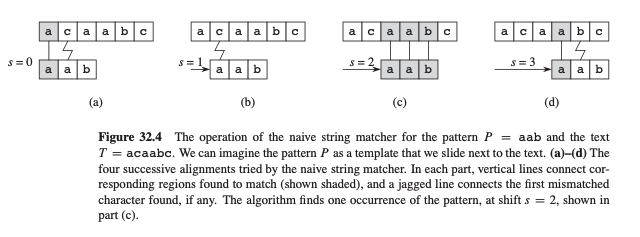
\includegraphics[width=0.7\textwidth]{naive-matching-algorithm}
    \caption{朴素字符串匹配算法}
    \label{naive-matching-algorithm}
  \end{figure}

  本次作业中基于朴素字符串匹配算法的实现具体可见下一节“判断依据”中的分析。

  \subsection*{判断依据}

  本程序打开目标文件后逐行读取,读取后调用函数lexicalAnalyse、逐行进行判断。

  函数lexicalAnalyse中有一静态变量is\_in\_comment,用于表示读取的该行代码是否处在跨行注释中,初始时该静态变量设为false。
\end{document}
